% بخش Docling - ابزار پردازش اسناد چندوجهی

\section{پردازش و نمایه‌سازی اسناد با \lr{Docling}}

\subsection{معرفی \lr{Docling}}
\lr{Docling} یک کتابخانه منبع‌باز پیشرفته برای پردازش و تبدیل اسناد ساختارنیافته به فرمت‌های قابل استفاده در سیستم‌های بازیابی اطلاعات است. این ابزار توسط تیم تحقیقاتی \lr{IBM} توسعه یافته و به‌صورت رایگان در دسترس جامعه علمی قرار گرفته است. \lr{Docling} با استفاده از مدل‌های یادگیری عمیق پیشرفته، قادر به تشخیص ساختار سلسله‌مراتبی اسناد، استخراج جداول پیچیده، و پردازش محتوای چندوجهی شامل متن، تصاویر و نمودارها می‌باشد.

\noindent
ویژگی‌های کلیدی \lr{Docling} عبارتند از:
\begin{itemize}
    \item \textbf{تشخیص ساختار سلسله‌مراتبی:} شناسایی خودکار عناوین، زیرعناوین، پاراگراف‌ها، و بخش‌های مختلف سند
    \item \textbf{استخراج دقیق جداول:} تبدیل جداول پیچیده با سلول‌های ادغام‌شده به فرمت ساختاریافته
    \item \textbf{پشتیبانی از محتوای چندوجهی:} پردازش همزمان متن، تصاویر، نمودارها و فرمول‌های ریاضی
    \item \textbf{خروجی استاندارد:} تولید فایل‌های \lr{JSON} ، \lr{YAML} و \lr{Markdown} با حفظ روابط والد-فرزندی بین عناصر
    \item \textbf{تکه‌سازی هوشمند:} ترکیب عناصر مرتبط در تکه‌های معنادار با رعایت محدودیت‌های طول توکن
\end{itemize}

\begin{figure}[!htbp]
    \centering
    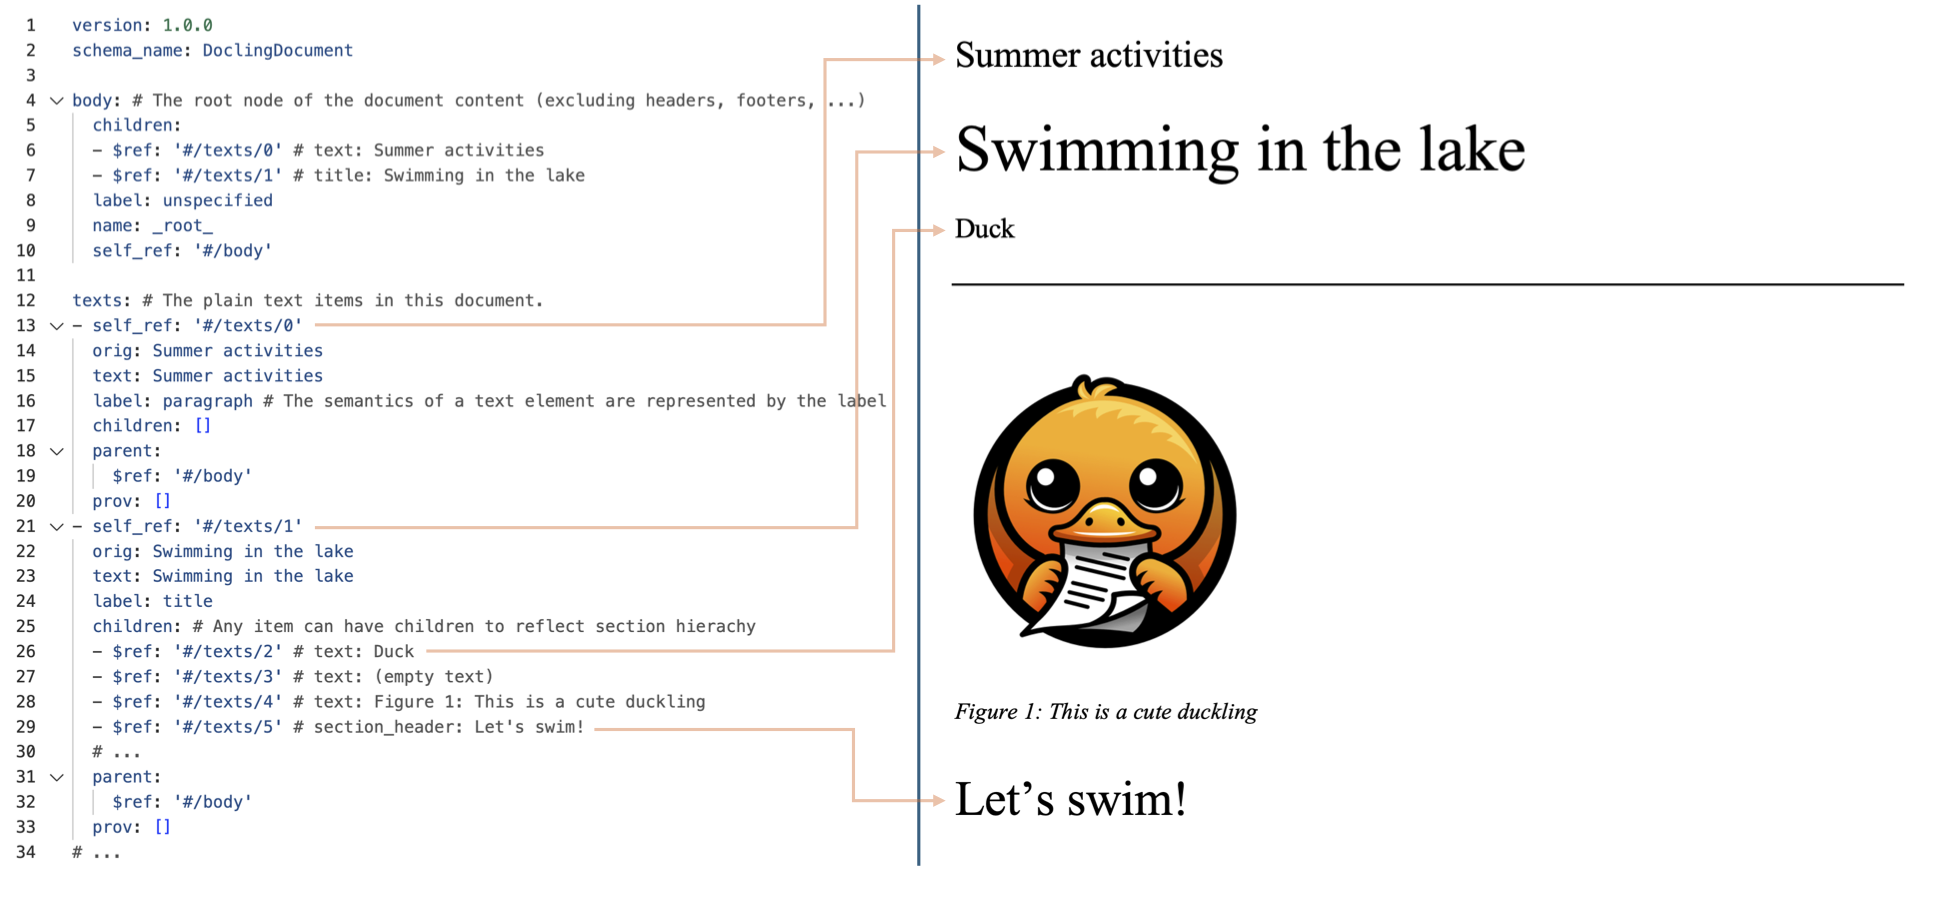
\includegraphics[width=0.95\textwidth]{docling_doc_hierarchy_1.png}
    \caption{نمونه‌ای از ساختار \lr{DoclingDocument}. سمت راست صفحه‌ای با عناوین، تصویر، زیرنویس و پاراگراف‌ها را نشان می‌دهد. سمت چپ درخت سند را نمایش می‌دهد که در آن هر عنصر با برچسب و اشاره‌گر خود در ساختار سلسله‌مراتبی قرار گرفته است.}
    \label{fig:docling_structure}
\end{figure}

\begin{figure}[!htbp]
    \centering
    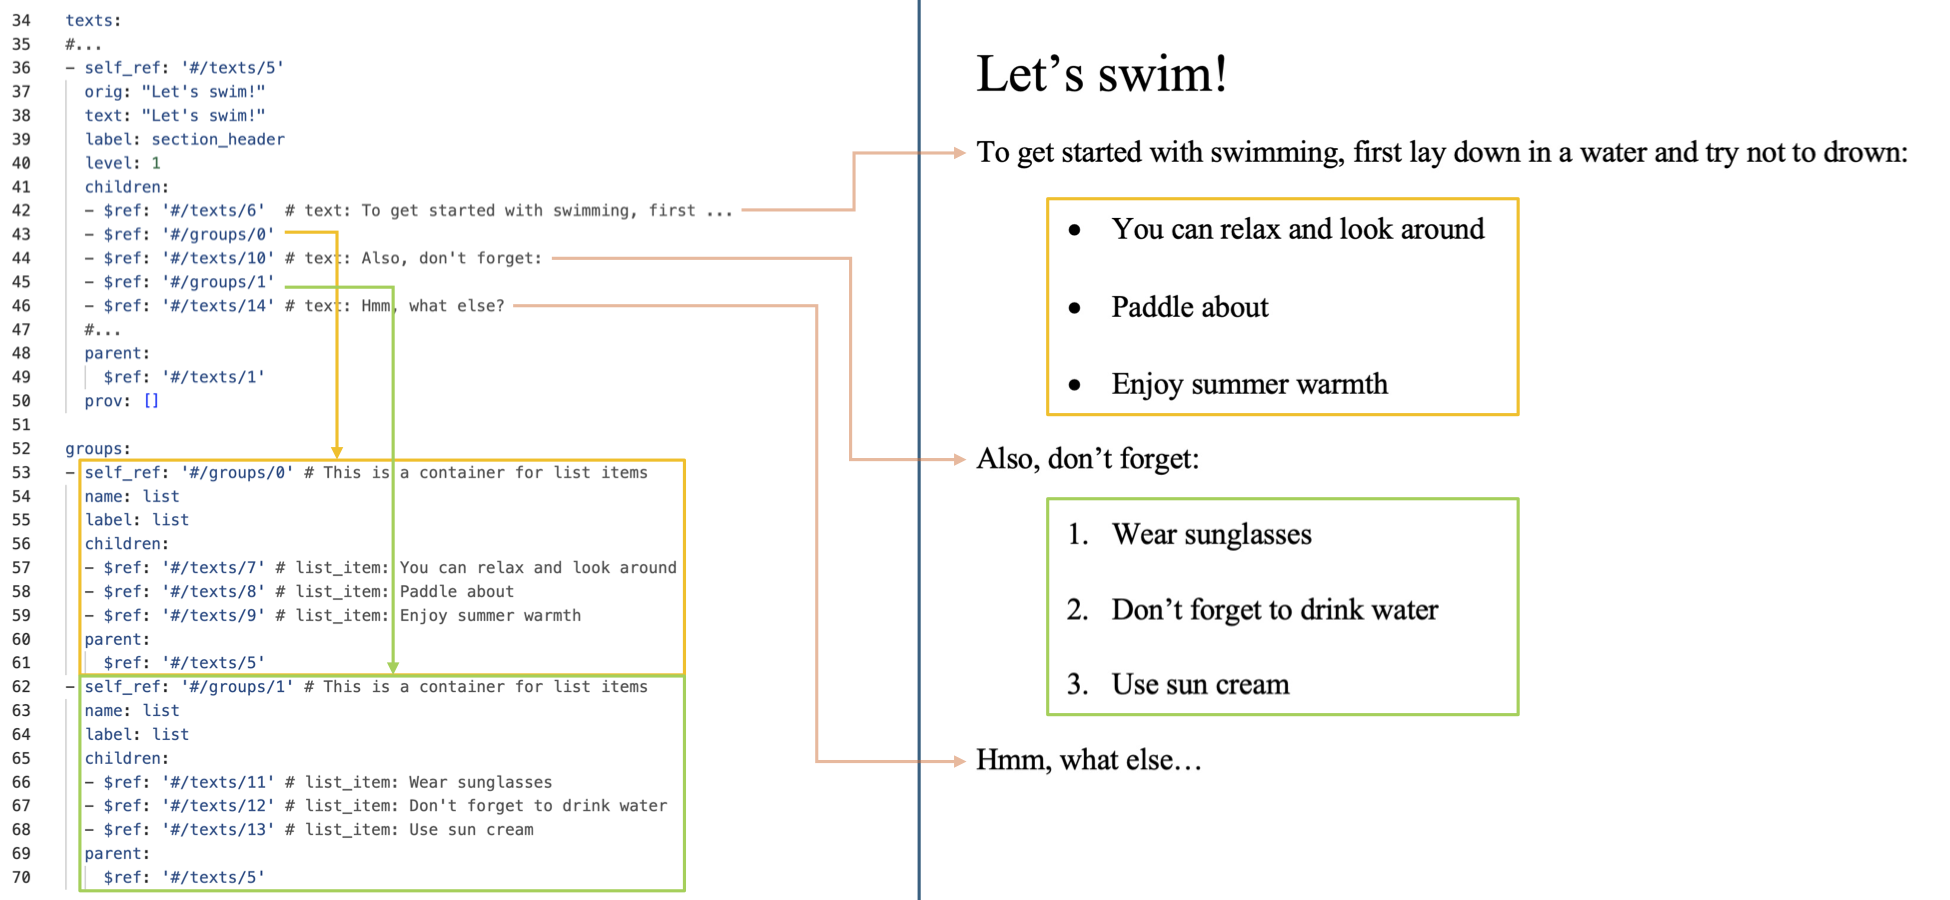
\includegraphics[width=0.95\textwidth]{docling_doc_hierarchy_2.png}
    \caption{فهرست‌های تو در تو و گروه‌ها در \lr{DoclingDocument}. سمت راست دو فهرست (یکی نقطه‌ای و دیگری شماره‌دار) را نشان می‌دهد. سمت چپ نشان می‌دهد که هر فهرست در یک کانتینر گروهی قرار می‌گیرد و عناصر آن به‌عنوان فرزند اضافه می‌شوند.}
    \label{fig:docling_groups}
\end{figure}

\subsection{دلایل انتخاب \lr{Docling}}
انتخاب \lr{Docling} به‌عنوان ابزار اصلی نمایه‌سازی کتاب پزشکی در این پروژه بر اساس ارزیابی دقیق نیازمندی‌های سیستم و مقایسه با ابزارهای موجود انجام شده است. در ادامه مهم‌ترین دلایل این انتخاب شرح داده می‌شود.

\subsubsection{پردازش اسناد پزشکی پیچیده}
اسناد پزشکی از پیچیده‌ترین انواع محتوای علمی هستند که شامل ترکیبی از متن تخصصی، جداول آماری، تصاویر تشخیصی، نمودارهای آناتومیکی و فرمول‌های دارویی می‌باشند. \lr{Docling} با معماری پردازشی چندمرحله‌ای خود، قادر به تشخیص و استخراج دقیق این عناصر متنوع است. برخلاف ابزارهای سنتی که صفحات را به‌صورت یک‌پارچه پردازش می‌کنند، \lr{Docling} از یک خط‌لوله مرحله‌ای استفاده می‌کند که در آن هر نوع محتوا با مدل تخصصی خود پردازش می‌شود.

\subsubsection{معماری مبتنی بر مدل‌های تخصصی}
یکی از برتری‌های اصلی \lr{Docling} نسبت به روش‌های مبتنی بر مدل‌های زبانی بزرگ چندوجهی \lr{(Vision Language Models)} این است که به‌جای استفاده از یک مدل عمومی برای تمام وظایف، از مدل‌های تخصصی برای هر بخش استفاده می‌کند:

\begin{itemize}
    \item \textbf{مدل تحلیل چیدمان (\lr{Layout Analysis}):} \lr{Docling} از مدل \lr{Heron} مبتنی بر معماری \lr{RT-DETR} با پشتوانه \lr{ResNet-50} استفاده می‌کند که روی مجموعه داده \lr{DocLayNet} شامل بیش از ۸۰ هزار صفحه برچسب‌گذاری شده آموزش دیده است. این مدل قادر به تشخیص ۱۷ کلاس مختلف شامل عنوان، متن، فهرست، جدول، تصویر، عنوان بخش، فرمول، زیرنویس و سایر عناصر است. دقت این مدل بر روی مجموعه داده استاندارد \lr{DocLayNet} به ۷۸ درصد \lr{mAP} می‌رسد (شکل \ref{fig:doclaynet_labels}).
\end{itemize}

\begin{figure}[!htbp]
    \centering
    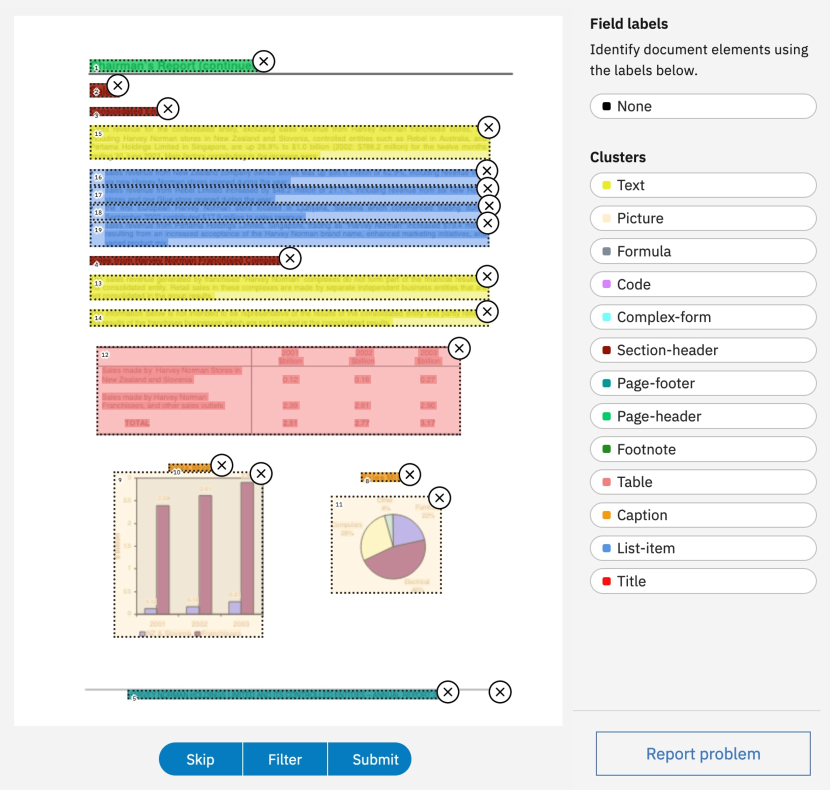
\includegraphics[width=0.65\textwidth]{doclaynet.png}
    \caption{نمونه‌ای از برچسب‌گذاری عناصر مختلف سند در مجموعه داده \lr{DocLayNet}. این تصویر نشان می‌دهد که چگونه هر عنصر صفحه (متن، عنوان، جدول، تصویر، فهرست و غیره) با کلاس‌های مختلف شناسایی و برچسب‌گذاری می‌شود. این برچسب‌های دقیق انسانی پایه آموزش مدل \lr{Heron} را تشکیل می‌دهند.}
    \label{fig:doclaynet_labels}
\end{figure}

\begin{itemize}
    \item \textbf{مدل استخراج ساختار جداول (\lr{TableFormer}):} برای پردازش جداول پیچیده، \lr{Docling} از مدل \lr{TableFormer} استفاده می‌کند که یک معماری ترنسفورمر مبتنی بر بینایی است. این مدل روی مجموعه داده‌های بزرگ شامل \lr{PubTabNet} (بیش از ۲۲۷ هزار جدول) آموزش دیده و قادر به تشخیص سطرها، ستون‌ها، سلول‌های ادغام‌شده، و ساختارهای پیچیده جداول است. خروجی این مدل شامل توالی توکن‌های \lr{HTML} و مختصات مرزی هر سلول است که سپس با متن اصلی \lr{PDF} تطبیق داده می‌شود (شکل \ref{fig:table_extraction}).
\end{itemize}

\begin{figure}[!htbp]
    \centering
    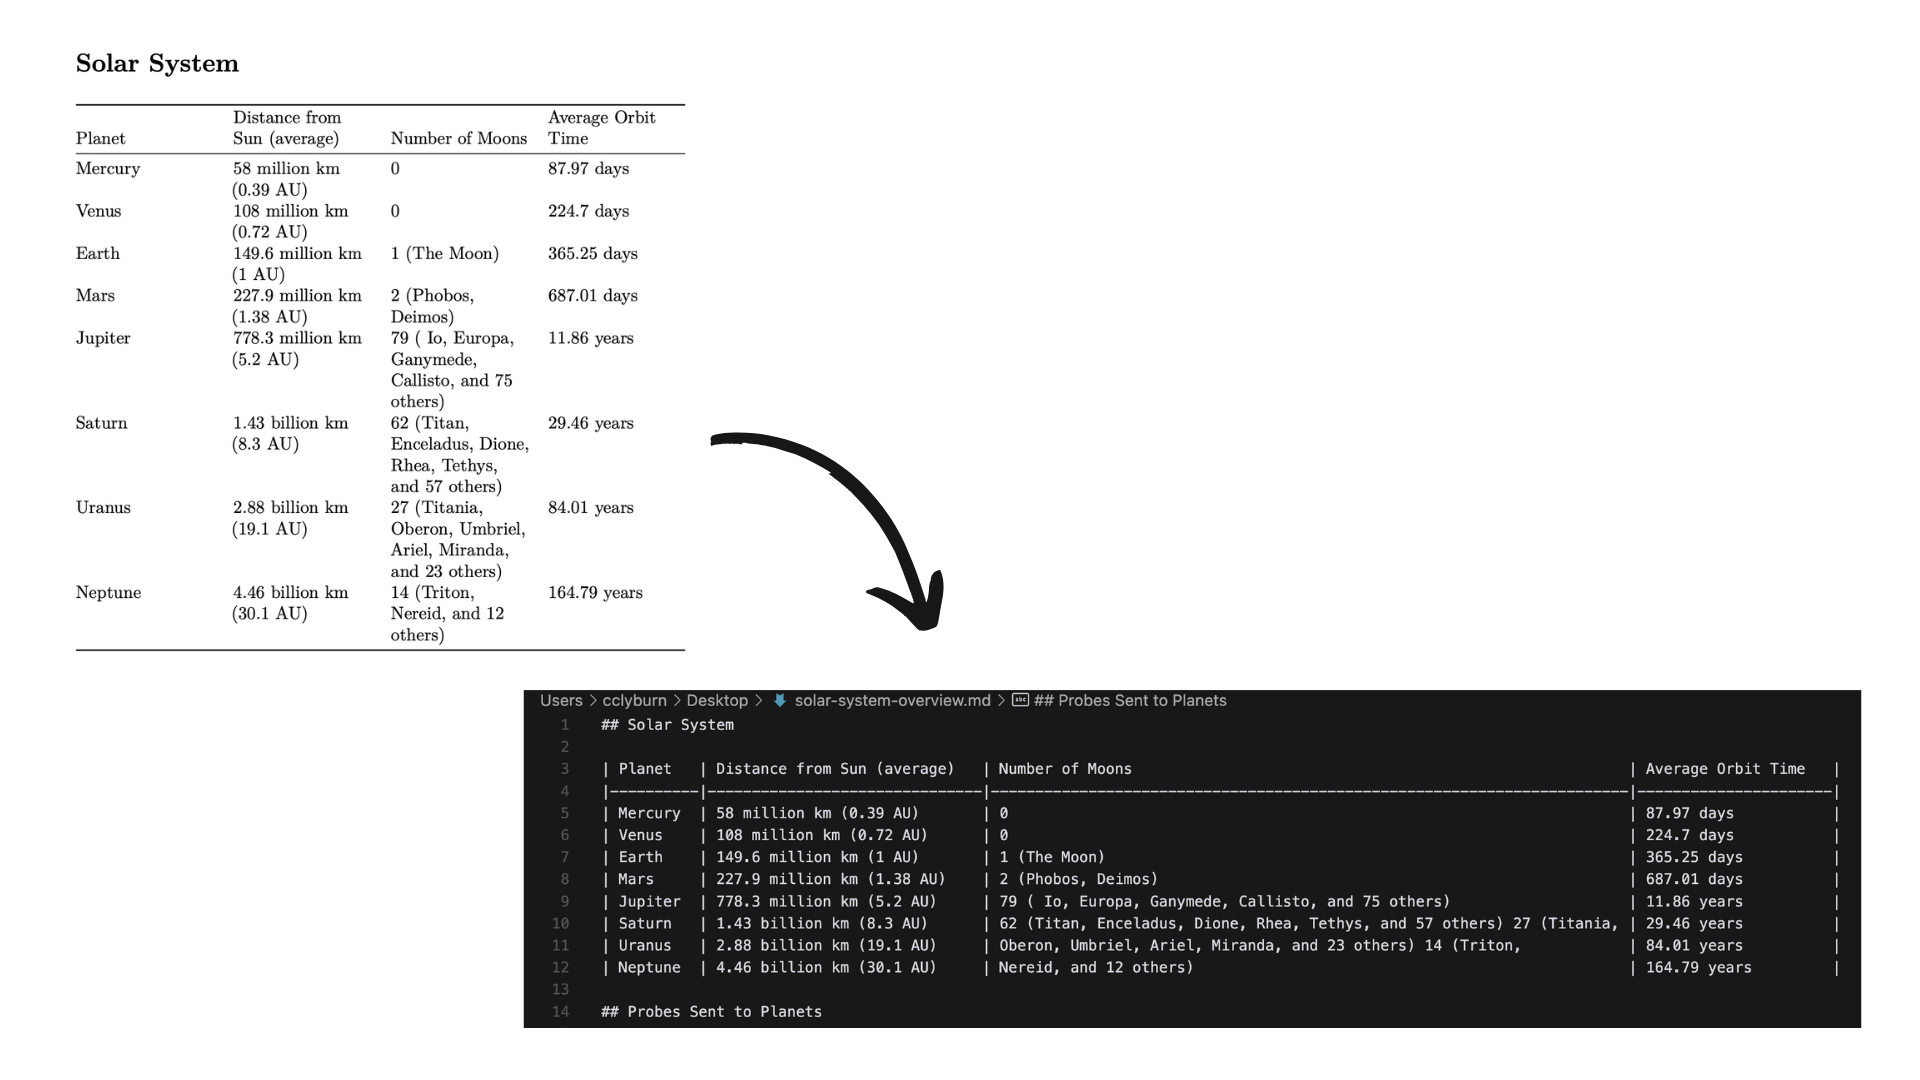
\includegraphics[width=0.85\textwidth]{docling_md_2.png}
    \caption{مثالی از استخراج دقیق جدول توسط \lr{TableFormer}. بالا: جدول اصلی منظم شامل اطلاعات سیارات منظومه شمسی. پایین: جدول استخراج شده در فرمت \lr{Markdown} که ساختار دقیق ستون‌ها و سطرها حفظ شده است.}
    \label{fig:table_extraction}
\end{figure}

\begin{itemize}
    \item \textbf{مدل توصیف تصاویر (\lr{Picture Description Model}):} یکی از چالش‌های مهم در پردازش کتاب‌های پزشکی، تولید توصیفات دقیق و جامع از تصاویر پیچیده پزشکی است. مدل پیش‌فرض \lr{Docling} برای این منظور \lr{SmolVLM} با حدود ۲۵۶ میلیون پارامتر است. با وجود سبک بودن این مدل، عملکرد آن در توصیف تصاویر پیچیده و نموداری پزشکی مطلوب نبود. در مرحله بعد، از مدل \lr{Granite-3.1 Vision} شرکت \lr{IBM} با ۲ میلیارد پارامتر استفاده شد که نتایج بهتری ارائه داد، اما به دلیل مشکل نشت حافظه \lr{(Memory Leak)} در \lr{Docling}، اجرای پایدار آن در محیط \lr{Google Colab} با \lr{GPU T4} امکان‌پذیر نبود. در نهایت، برای دستیابی به بهترین کیفیت توصیف، از \lr{API} رایگان مدل \lr{Gemini 2.5-Flash} شرکت \lr{Google} استفاده شد. برای مدیریت محدودیت‌های نرخ درخواست، یک سیستم تعویض خودکار بین توکن‌های مختلف پیاده‌سازی شد تا در صورت برخورد به خطای محدودیت نرخ با یک توکن، به‌طور خودکار از توکن دیگری استفاده شود و پردازش بدون وقفه ادامه یابد (شکل \ref{fig:picture_description}).
\end{itemize}

\begin{figure}[!htbp]
    \centering
    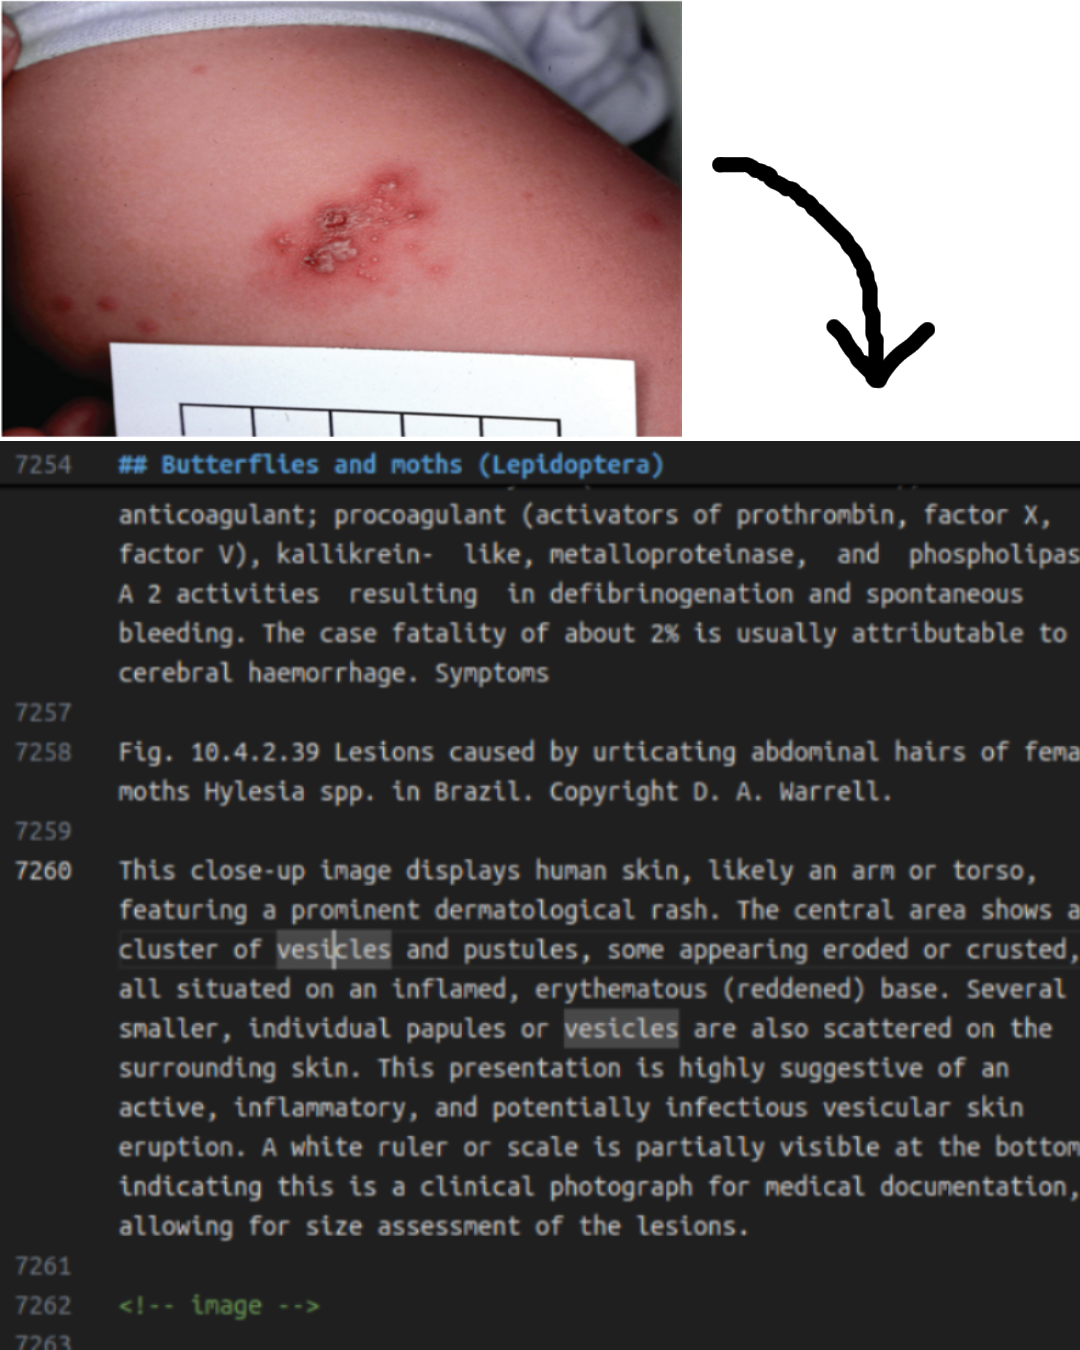
\includegraphics[width=0.95\textwidth]{picture_description.png}
    \caption{نمونه‌ای از خروجی مدل توصیف تصویر \lr{Gemini 2.5-Flash} برای یک تصویر پزشکی پیچیده. تصویر بالا یک ضایعه پوستی ناشی از تماس با موی بید برزیلی را نشان می‌دهد که شامل تاول‌ها و پاپول‌های قرمز روی پوست انسان است. مدل \lr{Gemini} توانسته است جزئیات کامل تصویر شامل نوع ضایعه، موقعیت آناتومیکی، و ویژگی‌های بالینی را به‌طور دقیق توصیف کند، که نشان‌دهنده برتری آن نسبت به مدل‌های سبک‌تر مانند \lr{SmolVLM} در پردازش تصاویر پزشکی پیچیده است.}
    \label{fig:picture_description}
\end{figure}

\begin{itemize}
    \item \textbf{موتور تشخیص نوشتار (\lr{OCR}):} برای پردازش محتوای اسکن‌شده یا تصویری، \lr{Docling} از \lr{EasyOCR} استفاده می‌کند که یک کتابخانه یادگیری عمیق مبتنی بر \lr{PyTorch} است. این موتور از مدل \lr{CRAFT} برای تشخیص مناطق متنی و مدل \lr{CRNN} برای خواندن کاراکترها استفاده می‌کند. \lr{Docling} صفحات را با وضوح ۲۱۶ \lr{DPI} رندر کرده و برای دستیابی به دقت بالا در تشخیص فونت‌های کوچک، از این موتور بهره می‌برد.
\end{itemize}

\noindent
این معماری متخصص‌محور باعث می‌شود دقت پردازش در مقایسه با مدل‌های عمومی چندوجهی به‌طور قابل توجهی افزایش یابد، زیرا هر مدل فقط بر روی یک وظیفه خاص تمرکز دارد و برای آن بهینه‌سازی شده است.

\subsubsection{حفظ ساختار سلسله‌مراتبی و روابط معنایی}
یکی از چالش‌های اساسی در پردازش اسناد پزشکی، حفظ روابط سلسله‌مراتبی بین عناصر مختلف است. کتاب‌های پزشکی دارای ساختار چندسطحی هستند که شامل فصل‌ها، بخش‌ها، زیربخش‌ها، پاراگراف‌ها، فهرست‌ها و عناصر وابسته مانند تصاویر و جداول می‌باشند. \lr{Docling} با استفاده از مدل ترتیب خواندن \lr{(Reading Order Model)} و سیستم مرجع‌دهی مبتنی بر \lr{JSON Pointer}، این روابط را به‌طور کامل حفظ می‌کند.

\noindent
در مدل داده \lr{DoclingDocument}، تمام عناصر در یک ساختار درختی سازماندهی می‌شوند که در آن:
\begin{itemize}
    \item هر عنصر دارای یک شناسه یکتا است
    \item روابط والد-فرزندی از طریق اشاره‌گرهای \lr{JSON} تعریف می‌شوند
    \item عناصر گروهی مانند فهرست‌ها در کانتینرهای مجزا نگهداری می‌شوند
    \item ترتیب طبیعی خواندن عناصر حفظ می‌شود
\end{itemize}

\noindent
این قابلیت برای سیستم بازیابی اطلاعات بسیار حیاتی است، زیرا امکان بازیابی محتوا با در نظر گرفتن بافت سلسله‌مراتبی آن را فراهم می‌کند. به‌عنوان مثال، هنگام بازیابی یک پاراگراف، سیستم می‌تواند به‌طور خودکار عنوان بخش و زیربخش مربوطه را نیز در نتایج قرار دهد.

\subsubsection{تکه‌سازی هوشمند با حفظ زمینه}
\lr{Docling} دارای یک سیستم تکه‌سازی هوشمند \lr{(Intelligent Chunker)} است که یکی از نقاط قوت اصلی این ابزار محسوب می‌شود. برخلاف روش‌های سنتی تکه‌سازی که صرفاً بر اساس تعداد کاراکتر یا پاراگراف عمل می‌کنند، تکه‌ساز \lr{Docling} از اطلاعات ساختاری سند برای ترکیب هوشمند عناصر مرتبط استفاده می‌کند.

\noindent
ویژگی‌های تکه‌ساز \lr{Docling}:
\begin{itemize}
    \item \textbf{ترکیب مبتنی بر معنا:} عناصر مرتبط مانند عنوان، پاراگراف‌های توضیحی، جداول و تصاویر مربوطه در یک تکه قرار می‌گیرند
    \item \textbf{رعایت محدودیت توکن:} تکه‌ها با توجه به حداکثر طول توکن مجاز ساخته می‌شوند
    \item \textbf{حفظ اطلاعات زمینه:} هر تکه شامل اطلاعات سلسله‌مراتبی مانند عنوان بخش و فصل است
    \item \textbf{جلوگیری از شکستگی محتوا:} جداول و فهرست‌ها به‌صورت یک‌پارچه در تکه‌ها قرار می‌گیرند
\end{itemize}

\noindent
این رویکرد باعث می‌شود که تکه‌های تولید شده از نظر معنایی منسجم و برای سیستم بازیابی قابل استفاده باشند.

\subsubsection{خروجی استاندارد و قابل پردازش}
\lr{Docling} دو نوع خروجی اصلی ارائه می‌دهد که هر کدام برای کاربردهای خاصی مناسب هستند:

\begin{itemize}
    \item \textbf{فرمت \lr{Markdown}:} نسخه تمیز و خوانا از سند که در آن ساختار سلسله‌مراتبی با استفاده از سرفصل‌های \lr{Markdown} (مثل \lr{\#}, \lr{\#\#}, \lr{\#\#\#}) نمایش داده می‌شود، جداول به‌صورت جداول \lr{Markdown} فرمت می‌شوند، و محتوای متنی به‌صورت پاراگراف‌های منظم سازماندهی می‌شود.
    
    \item \textbf{فرمت \lr{JSON}:} نمایش کامل و ساختاریافته سند که شامل تمام متادیتا، روابط سلسله‌مراتبی، مختصات عناصر، و اطلاعات تکمیلی است. این فرمت برای پردازش خودکار و نمایه‌سازی در پایگاه‌های داده بسیار مناسب است.
\end{itemize}

\noindent
در این پروژه، از فرمت \lr{JSON} برای استخراج دقیق اطلاعات و نمایه‌سازی در \lr{Elasticsearch} استفاده می‌شود، در حالی که فرمت \lr{Markdown} برای بازبینی انسانی و کنترل کیفیت مورد استفاده قرار می‌گیرد.

\subsubsection{منبع‌باز و قابل توسعه}
\lr{Docling} به‌صورت کامل منبع‌باز و تحت مجوز \lr{MIT} منتشر شده است که مزایای زیر را به همراه دارد:

\begin{itemize}
    \item امکان بررسی و درک کامل نحوه عملکرد داخلی سیستم
    \item قابلیت سفارشی‌سازی و توسعه مدل‌ها برای نیازهای خاص
    \item کاهش هزینه‌های عملیاتی با حذف نیاز به \lr{API‌های} پولی
    \item امکان اجرا در محیط‌های محلی و امن
\end{itemize}

\noindent
این ویژگی برای پروژه‌های پزشکی که با داده‌های حساس سر و کار دارند، بسیار حیاتی است.

\subsubsection{کارایی و سرعت پردازش}
\lr{Docling} با استفاده از بهینه‌سازی‌های مختلف، سرعت پردازش قابل قبولی را ارائه می‌دهد:

\begin{itemize}
    \item استفاده از \lr{ONNX Runtime} برای استنتاج سریع‌تر مدل‌ها
    \item پردازش موازی صفحات در صورت وجود منابع کافی
    \item استفاده از رزولوشن مناسب برای هر مرحله (۷۲ \lr{DPI} برای تحلیل چیدمان و ۲۱۶ \lr{DPI} برای \lr{OCR})
    \item کش کردن نتایج میانی برای جلوگیری از پردازش مجدد
\end{itemize}

\noindent
در آزمایش‌های انجام شده بر روی کتاب پزشکی مورد استفاده در این پروژه، \lr{Docling} توانست هر صفحه را در زمان متوسط ۱۰ تا ۱۵ ثانیه (با \lr{GPU T4} در محیط \lr{Google Colab}) پردازش کند که برای کاربردهای دسته‌ای قابل قبول است.

\subsubsection{یکپارچگی با ابزارهای پردازش زبان طبیعی}
\lr{Docling} به‌راحتی با کتابخانه‌های پردازش زبان طبیعی و سیستم‌های بازیابی یکپارچه می‌شود. در این پروژه، خروجی \lr{Docling} به‌طور مستقیم به \lr{Elasticsearch} منتقل می‌شود و با استفاده از \lr{LangChain} برای ایجاد زنجیره‌های پردازشی پیچیده‌تر استفاده می‌شود. این یکپارچگی آسان امکان ساخت خط‌لوله‌های پردازشی پیچیده را با حداقل کد اضافی فراهم می‌کند.

\subsection{مقایسه با روش‌های جایگزین}
برای ارزیابی جامع‌تر انتخاب \lr{Docling}، مقایسه‌ای با سایر روش‌های موجود انجام شده است:

\subsubsection{مدل‌های زبانی بزرگ چندوجهی \lr{(Vision Language Models)}}
مدل‌هایی مانند \lr{OpenAI GPT}، \lr{Claude 4}، و \lr{Gemini} قادر به پردازش تصاویر صفحات هستند، اما محدودیت‌های زیر را دارند:

\begin{itemize}
    \item \textbf{هزینه بالا:} هر صفحه نیاز به فراخوانی \lr{API} دارد که برای کتاب‌های بزرگ هزینه‌بر است
    \item \textbf{عدم تضمین ساختار:} خروجی این مدل‌ها ممکن است فاقد ساختار ثابت باشد. مقایسه‌ای از عملکرد پایپلاین آماده شده با داکلینگ و GPT-5 در \href{https://github.com/Alijanloo/MultiModalRag/tree/master/docs/compare\%20docling\%20with\%20GPT-5}{این آدرس} تهیه شده است.
    \item \textbf{محدودیت در جداول پیچیده:} دقت پایین در استخراج جداول با ساختار پیچیده
\end{itemize}


\subsubsection{کتابخانه‌های سنتی \lr{PDF} مانند \lr{PyPDF2} و \lr{PDFMiner}}
این ابزارها فقط متن برنامه‌نویسی‌شده \lr{PDF} را استخراج می‌کنند و محدودیت‌های اساسی دارند:

\begin{itemize}
    \item عدم تشخیص ساختار سلسله‌مراتبی
    \item ناتوانی در پردازش جداول پیچیده
    \item عدم پشتیبانی از محتوای اسکن‌شده
    \item خروجی بدون ساختار و فاقد متادیتا
\end{itemize}

\subsubsection{مقایسه با \lr{Unstructured.io}}
یکی از جدیدترین و قدرتمندترین جایگزین‌های تجاری برای \lr{Docling}، پلتفرم \lr{Unstructured.io} است که به‌صورت ترکیبی از نسخه منبع‌باز و سرویس ابری ارائه می‌شود. این پلتفرم نیز هدف مشابهی با \lr{Docling} دارد: تبدیل اسناد ساختارنیافته به داده‌های قابل استفاده برای سیستم‌های هوش مصنوعی.

\noindent
ویژگی‌های کلیدی \lr{Unstructured.io}:
\begin{itemize}
    \item \textbf{تجزیه و تقسیم‌بندی پیشرفته:} قابلیت شناسایی و جداسازی عناصر مختلف سند شامل پاراگراف‌ها، جداول، عناوین و تصاویر
    \item \textbf{تمیزسازی و بهنجارسازی:} حذف نویزها و نرمال‌سازی محتوا برای کیفیت بهتر پردازش
    \item \textbf{تکه‌سازی انطباقی:} تقسیم محتوا به تکه‌های مناسب برای ورودی مدل‌های زبانی
    \item \textbf{کانکتورهای یکپارچه‌سازی:} اتصال مستقیم به پایگاه‌های داده، دریاچه‌های داده و سیستم‌های ذخیره‌سازی
\end{itemize}


\noindent
\lr{Unstructured.io} برای پروژه‌هایی که بودجه کافی برای سرویس‌های ابری موجود است، و اولویت بالایی برای سرعت پیاده‌سازی نسبت به کنترل کامل فرآیند قائل هستند، گزینه مناسبی محسوب می‌شود.

\noindent
با توجه به این مقایسه، \lr{Docling} ترکیبی بهینه از دقت، کارایی، انعطاف‌پذیری و هزینه را ارائه می‌دهد که برای پردازش کتاب‌های پزشکی ایده‌آل است.

\newpage

\subsection{یکپارچگی با سیستم نمایه‌سازی}
در این پروژه، خروجی \lr{Docling} به‌صورت زیر با سیستم نمایه‌سازی یکپارچه می‌شود:

\begin{enumerate}
    \item \textbf{دریافت \lr{DoclingDocument}:} پس از پردازش \lr{PDF}، شی \lr{DoclingDocument} حاوی تمام اطلاعات ساختاریافته دریافت می‌شود
    
    \item \textbf{تکه‌سازی هوشمند:} با استفاده از \lr{HybridChunker} داخلی \lr{Docling}، سند به تکه‌های معنادار با حداکثر طول توکن مشخص تقسیم می‌شود
    
    \item \textbf{غنی‌سازی با متادیتا:} هر تکه با اطلاعات اضافی شامل عنوان بخش، شماره صفحه، نوع محتوا، و روابط سلسله‌مراتبی غنی می‌شود
    
    \item \textbf{پردازش تصاویر:} تصاویر استخراج‌شده به مدل \lr{Gemini 2.5-Flash} ارسال می‌شوند تا توصیف دقیق و جامعی از آن‌ها تولید شود
    
    \item \textbf{نمایه‌سازی در \lr{Elasticsearch}:} تکه‌های نهایی به همراه توصیف تصاویر و متادیتای کامل در \lr{Elasticsearch} نمایه‌سازی می‌شوند
\end{enumerate}

\subsection{نتیجه‌گیری}
با توجه به ویژگی‌های منحصر به فرد \lr{Docling} از جمله معماری مبتنی بر مدل‌های تخصصی، حفظ ساختار سلسله‌مراتبی، تکه‌سازی هوشمند، و ماهیت منبع‌باز آن، این ابزار به‌عنوان بهترین انتخاب برای نمایه‌سازی کتاب پزشکی در این پروژه شناسایی شد. ترکیب \lr{Docling} با مدل چندوجهی \lr{Gemini} برای توصیف تصاویر و \lr{Elasticsearch} برای ذخیره‌سازی و بازیابی، یک سیستم جامع و کارآمد برای بازیابی اطلاعات پزشکی ایجاد می‌کند که قادر به پاسخگویی به پرسش‌های پیچیده با استفاده از اطلاعات متنی، جدولی و تصویری است.
